\let\negmedspace\undefined
\let\negthickspace\undefined
\documentclass[journal]{IEEEtran}
\usepackage[a5paper, margin=10mm, onecolumn]{geometry}
%\usepackage{lmodern} % Ensure lmodern is loaded for pdflatex
\usepackage{tfrupee} % Include tfrupee package

\setlength{\headheight}{1cm} % Set the height of the header box
\setlength{\headsep}{0mm}     % Set the distance between the header box and the top of the text

\usepackage{gvv-book}
\usepackage{gvv}
\usepackage{cite}
\usepackage{amsmath,amssymb,amsfonts,amsthm}
\usepackage{algorithmic}
\usepackage{graphicx}
\usepackage{textcomp}
\usepackage{xcolor}
\usepackage{txfonts}
\usepackage{listings}
\usepackage{enumitem}
\usepackage{mathtools}
\usepackage{gensymb}
\usepackage{comment}
\usepackage[breaklinks=true]{hyperref}
\usepackage{tkz-euclide} 
\usepackage{listings}
% \usepackage{gvv}                                        
\def\inputGnumericTable{}                                 
\usepackage[latin1]{inputenc}                                
\usepackage{color}                                            
\usepackage{array}                                            
\usepackage{longtable}                                       
\usepackage{calc}                                             
\usepackage{multirow}                                         
\usepackage{hhline}                                           
\usepackage{ifthen}
\usepackage{lscape}
\begin{document}

\bibliographystyle{IEEEtran}



\title{2.9.8}
\author{EE25BTECH11057 - Rushil Shanmukha Srinivas
}
% \maketitle
% \newpage
% \bigskip
{\let\newpage\relax\maketitle}

\renewcommand{\thefigure}{\theenumi}
\renewcommand{\thetable}{\theenumi}
\setlength{\intextsep}{10pt} % Space between text and floats

\numberwithin{equation}{enumi}
\numberwithin{figure}{enumi}
\renewcommand{\thetable}{\theenumi}

\textbf{Question} : $\vec a,\vec b,\vec c ,\vec d $ are four non-zero vectors such that
$\vec a \times \vec b = \vec c \times \vec d$ and $ \vec a \times \vec c = 4\,\vec b \times \vec d$
then show that $(\vec a - 2\vec d)$ is parallel to $(2\vec b - \vec c)$ where $\vec a \neq 2\vec d $ , $\vec c \neq 2\vec b.$
\newline
\textbf{Solution} :
We are given nonzero vectors $\vec a,\vec b,\vec c,\vec d $ such that
\begin{align}
\vec a\times \vec b = \vec c\times \vec d,
\vec a\times \vec c = 4\,\vec b\times \vec d,
\end{align}
with $\vec a\neq 2\vec d$ and $\vec c\neq 2\vec b$.

We need to show $(\vec a- 2\vec d)$ is parallel to $(2\vec b-\vec c)$, i.e.
\begin{align}
(\mathbf a-2\mathbf d)\times(2\mathbf b-\mathbf c)=\mathbf0.
\end{align}
By bilinearity:
\begin{align}
(\vec a-2\vec d)\times(2\vec b-\vec c)
= 2(\vec a\times\vec b) - (\vec a\times\vec c)
 - 4(\vec d\times\vec b) + 2(\vec d\times\vec c).
\end{align}

Also, $\vec d\times\vec b=-\vec b\times\vec d$ and
$\vec d\times\vec c=-\vec c\times\vec d$.

Substitute these:
\begin{align}
&2(\vec c\times\vec d) - 4(\vec b\times\vec d)
   -4(-\vec b\times\vec d) + 2(-\vec c\times\vec d) \\
&= 2(\vec c\times\vec d) - 4(\vec b\times\vec d)
   + 4(\vec b\times\vec d) - 2(\vec c\times\vec d) = \vec 0.
\end{align}


Let $\vec u=\vec a-2\vec d$ and $\vec v=2\vec b-\vec c$.  
Since $\vec u\times \vec v=\vec 0$, they are linearly dependent.

Equivalently, the matrix
\begin{align}
M = [\,\mathbf u \ \ \mathbf v\,]
\end{align}
has $\operatorname{rank}(M)=1$.
 This is exactly the criterion for $\vec u$ and $\vec v$ to be parallel.

Therefore,
\begin{align}
\boxed{\,\vec a-2\vec d \parallel 2\vec b-\vec c\,}.
\end{align}

\begin{figure}[h!]
  \centering
  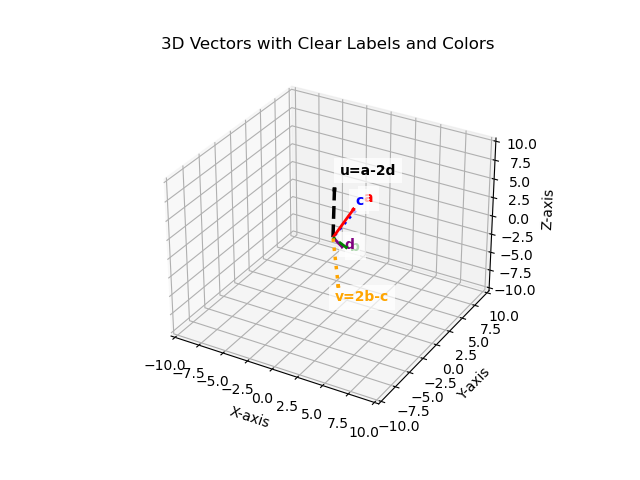
\includegraphics[width=0.9\columnwidth]{figs/fig4.png} 
   \caption*{Fig: Representation of vectors}
  \label{Fig4}
\end{figure}

\end{document}
